\documentclass[11pt,a4paper]{article}

\usepackage[utf8]{inputenc}
\usepackage[T1]{fontenc}
\usepackage[french]{babel}
\usepackage{lmodern}
\usepackage[a4paper,margin=2.5cm]{geometry}
\usepackage{graphicx}
\usepackage{booktabs}
\usepackage{array}
\usepackage{listings}
\usepackage{xcolor}
\usepackage[hidelinks]{hyperref}
\usepackage{caption}

\hypersetup{
  pdftitle={Surfaces implicites et distances signées},
  pdfauthor={À compléter}
}

\setlength{\parskip}{0.4em}
\setlength{\parindent}{0pt}
\captionsetup{font=small,labelfont=bf}

\newcommand{\todo}[1]{\textbf{[À compléter : #1]}}
\newcommand{\placeholderfigure}[2]{%
  \begin{figure}[htbp]
    \centering
    \fbox{\parbox[c][5cm][c]{0.82\textwidth}{\centering #2}}
    \caption{#1}
  \end{figure}
}

\lstset{
  basicstyle=\ttfamily\small,
  breaklines=true,
  frame=single,
  numbers=left,
  numberstyle=\tiny,
  showstringspaces=false
}

\title{
  Surfaces implicites\\
  \large Projet d'informatique graphique
}
\author{\todo{nom(s) et prénom(s)}}
\date{Master 2 Informatique -- 2026--2027}

\begin{document}

\maketitle
\tableofcontents

\section{Introduction}
\subsection{Objectifs et réalisations}
\todo{Présenter les deux méthodes de visualisation utilisées. Le marching cubes échantillonne le champ sur une grille, extrait un maillage puis le rend avec OpenGL. Le sphere tracing évalue le champ le long des rayons de la caméra et affiche directement la surface, ici dans un fragment shader. Comparer brièvement leurs principes et les paramètres qui influencent le résultat.}


\subsection{Visualisation des surfaces}
\todo{Présenter les deux méthodes de visualisation utilisées. Le marching cubes échantillonne le champ sur une grille, extrait un maillage puis le rend avec OpenGL. Le sphere tracing évalue le champ le long des rayons de la caméra et affiche directement la surface, ici dans un fragment shader. Comparer brièvement leurs principes et les paramètres qui influencent le résultat.}

\subsection{Mesures de performances}
Les mesures sont faites sur un Intel Core i5-11400H (Ubuntu~24.04, g++~13.3, compilation Release \texttt{-O3}, un seul thread). Chaque temps est la médiane de 5~mesures, prises avec \texttt{std::chrono::steady\_clock}.
\todo{Compléter pour les expériences des autres sections (scènes, nombre d'appels).}
Il est important de prendre en compte la distance de la camera lors de l'evaluation des performances car c'est un facteur qui agit directement sur le nombre de pixels et donc de rayon qui touchent et/ou sont proche de la surface ce qui veut dire plus d'appels à Value.
\section{Modélisation par SDF}
\subsection{Arbre de construction}
\todo{Présenter la construction d'une scène à partir de primitives et d'opérateurs. Ajouter un exemple d'arbre utilisé dans le projet.}

\subsection{Primitives}
\todo{Présenter les primitives implémentées, leurs paramètres et leurs formules. Ne garder que celles qui fonctionnent.}

\subsection{Opérateurs et transformations}
\todo{Décrire les opérateurs effectivement disponibles : union, intersection, soustraction, mélange lisse, répétition, torsion et bruit, selon le périmètre réellement validé.}

\subsection{Résultats et performances}
\placeholderfigure{Maillage généré à partir d'un arbre SDF}{Insérer une capture du maillage et préciser la scène, la résolution et les paramètres.}
\todo{Commenter le rendu et la qualité du maillage pour les scènes testées.}
\begin{table}[htbp]
  \centering
  \caption{Temps d'évaluation des différentes primitives et opérations.}
  \label{tab:sdf-performance}
  \small
  \begin{tabular}{lrrr}
    \toprule
    Scène ou primitive & \shortstack{Nombre\\d'appels} & \shortstack{Temps\\(ms)} & \shortstack{Moyenne\\(ns)} \\
    \midrule
    Sphère & \ldots & \ldots & \ldots \\
    Boîte & \ldots & \ldots & \ldots \\
    Arbre composé & \ldots & \ldots & \ldots \\
    \bottomrule
  \end{tabular}
\end{table}

\todo{Renseigner les temps mesurés, le nombre d'appels (notamment $10^7$ si ce protocole a été utilisé) et commenter les écarts observés.}

\section{Érosion procédurale}
L'objectif est de simuler le vieillissement d'un objet : on projette sur lui des sphères qui creusent localement sa surface. Toute l'érosion est faite côté CPU sur l'arbre C++ (fichiers \texttt{SI/erosion.hpp} et \texttt{SI/erosion.cpp}) ; les mesures sont dans un programme séparé (\texttt{erosion\_benchmark.cpp}).

\subsection{Intersection rayon--SDF}
L'intersection est la méthode \texttt{bool NodeSDF::Intersect(const Ray\& ray, double\& t, double tMax, double eps, int maxSteps) const}, disponible pour tous les nœuds de l'arbre. Elle utilise le sphere tracing : en un point $p$, la valeur $d = f(p)$ du champ est la distance à la surface la plus proche, donc on peut avancer de $d$ le long du rayon sans traverser la surface.

On part de l'origine du rayon ($t = 0$) puis, à chaque itération :
\begin{enumerate}
  \item on calcule $p = o + t\,\vec{u}$ et $d = f(p)$ ;
  \item si $d < \varepsilon$ ($\varepsilon = 10^{-4}$), on est sur la surface : on renvoie \texttt{true} et $t$ contient la distance d'impact ;
  \item sinon on avance : $t \leftarrow t + d$ ;
  \item si $t > t_{\max}$ ($t_{\max} = 100$), le rayon est sorti de la scène : on renvoie \texttt{false}.
\end{enumerate}
Au-delà de 256 itérations, on considère aussi qu'il n'y a pas d'impact. La direction $\vec{u}$ doit être normalisée, sinon $t$ n'est plus une distance. L'origine doit être hors de l'objet.

\subsection{Algorithme d'érosion}
\subsubsection{Projection des impacts}
Les projectiles partent d'une sphère englobante de centre $c$ et de rayon $R$ qui contient l'objet. Pour chaque projectile, on tire une direction $\vec{v}$ uniforme sur la sphère unité (tirage par rejet : un point uniforme dans le cube $[-1,1]^3$ est gardé s'il est dans la boule unité, puis normalisé). Le rayon part de $c + R\,\vec{v}$ et vise le centre, avec la direction $-\vec{v}$.

Si le rayon touche l'objet en $t$, on crée une sphère de rayon $r$ (le cratère) centrée au point d'impact, et on la soustrait à l'objet avec l'opérateur de soustraction : $f \leftarrow \max(f, -f_{\text{sphère}})$. Le générateur pseudo-aléatoire est initialisé avec une graine : à graine égale, les deux méthodes ci-dessous tirent exactement les mêmes rayons, ce qui permet de les comparer.

\subsubsection{Érosion incrémentale et par paquets}
\paragraph{Incrémentale.} Chaque cratère est soustrait dès qu'il est créé. Le rayon suivant est donc lancé sur l'objet déjà creusé, et il peut tomber au fond d'un cratère précédent pour creuser plus profond. L'arbre obtenu est une chaîne de $n$ soustractions :
\[
  \mathrm{Sub}(\dots\mathrm{Sub}(\mathrm{Sub}(\text{objet}, s_0), s_1)\dots, s_{n-1}).
\]

\paragraph{Par paquets.} Les rayons sont regroupés par paquets de $k$. Les $k$ rayons d'un paquet sont tous lancés sur le même objet, celui d'avant le paquet. Leurs cratères sont ensuite réunis dans un arbre d'unions équilibré (fonction \texttt{MakeUnionTree}, profondeur $\lceil\log_2 k\rceil$), qui est soustrait en une seule fois :
\[
  \mathrm{Sub}(\dots\mathrm{Sub}(\text{objet}, \mathrm{Union}(\text{paquet}_0))\dots, \mathrm{Union}(\text{paquet}_{\lceil n/k\rceil-1})).
\]
Les rayons d'un même paquet ne voient donc pas les cratères les uns des autres. Pour $k = 1$, on retrouve exactement l'arbre incrémental.

Dans les deux cas, si les $n$ rayons touchent l'objet, l'arbre contient $n$ sphères et $2n+1$ nœuds. Seule sa forme change : l'arbre incrémental a une profondeur $n+1$, l'arbre par paquets une profondeur $\lceil n/k\rceil + \lceil\log_2 k\rceil + 1$.

\subsection{Résultats}
\paragraph{Protocole.} L'objet est une boîte de demi-côtés 0,5, les cratères ont un rayon de 0,05, et la même graine est utilisée pour toutes les méthodes, qui tirent donc les mêmes rayons. On fait varier le nombre d'impacts $n$ de 100 à 4000 et la taille des paquets $k$ de 5 à 500. Pour chaque configuration, on mesure le temps de \textbf{construction} de l'objet érodé et le temps d'un appel à \textbf{\texttt{Value}} sur l'objet final. La précision est comparée visuellement.

\begin{table}[htbp]
  \centering
  \caption{Temps de construction (ms) selon le nombre d'impacts $n$ et la taille des paquets $k$.}
  \label{tab:erosion-construction}
  \small
  \begin{tabular}{rrrrrrrr}
    \toprule
    $n$ & Incrémentale & $k=5$ & $k=10$ & $k=25$ & $k=50$ & $k=100$ & $k=500$ \\
    \midrule
    100  & 0,27 & 0,14 & 0,13 & 0,11 & 0,09 & & \\
    500  & 8,34 & 4,12 & 3,59 & 3,25 & 2,99 & 2,64 & \\
    1000 & 42,7 & 20,9 & 18,5 & 16,4 & 15,6 & 14,5 & 6,94 \\
    2000 & 223  & 111  & 99,3 & 89,6 & 85,0 & 81,1 & 54,5 \\
    4000 & 1618 & 824  & 754  & 673  & 608  & 569  & 356 \\
    \bottomrule
  \end{tabular}
\end{table}

\begin{table}[htbp]
  \centering
  \caption{Temps d'un appel à \texttt{Value} sur l'objet final ($\mu$s).}
  \label{tab:erosion-value}
  \small
  \begin{tabular}{rrrrrrrr}
    \toprule
    $n$ & Incrémentale & $k=5$ & $k=10$ & $k=25$ & $k=50$ & $k=100$ & $k=500$ \\
    \midrule
    100  & 0,86 & 0,41 & 0,37 & 0,37 & 0,38 & & \\
    500  & 4,44 & 2,21 & 1,92 & 1,79 & 1,69 & 1,69 & \\
    1000 & 9,10 & 4,53 & 4,08 & 3,74 & 3,55 & 3,52 & 3,51 \\
    2000 & 18,0 & 8,86 & 8,17 & 7,44 & 7,17 & 6,98 & 7,06 \\
    4000 & 34,6 & 19,2 & 17,3 & 14,9 & 14,3 & 14,0 & 14,0 \\
    \bottomrule
  \end{tabular}
\end{table}

\begin{table}[htbp]
  \centering
  \caption{Gain des paquets par rapport à l'érosion incrémentale pour $n = 4000$.}
  \label{tab:erosion-synthese}
  \small
  \begin{tabular}{lrrrrrr}
    \toprule
    $k$ & 5 & 10 & 25 & 50 & 100 & 500 \\
    \midrule
    Construction   & $\times$2,0 & $\times$2,1 & $\times$2,4 & $\times$2,7 & $\times$2,8 & $\times$4,5 \\
    \texttt{Value} & $\times$1,8 & $\times$2,0 & $\times$2,3 & $\times$2,4 & $\times$2,5 & $\times$2,5 \\
    \bottomrule
  \end{tabular}
\end{table}

\begin{figure}[htbp]
  \centering
  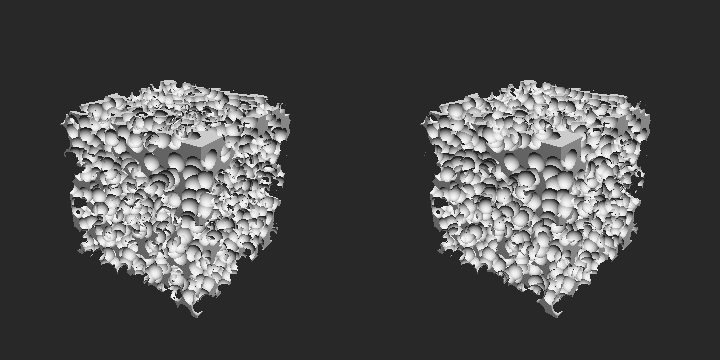
\includegraphics[width=0.85\textwidth]{figures/erosion_rendu.png}
  \caption{Rendu par sphere tracing des deux objets érodés, $n = 2000$ impacts : érosion incrémentale à gauche, paquets de $k = 500$ à droite.}
  \label{fig:erosion-rendu}
\end{figure}

\subsubsection{Analyse : incrémental contre paquets}

\paragraph{Incrémentale : plus précise, mais plus longue.} Chaque rayon est lancé sur l'objet déjà creusé par tous les impacts précédents. Un projectile qui tombe dans un cratère creuse donc plus profond : c'est le comportement attendu d'une érosion, et c'est la référence de précision. En contrepartie, l'arbre est une chaîne de $n$ soustractions, très profonde :
\begin{itemize}
  \item la construction coûte cher, car le rayon $i$ doit parcourir un arbre qui contient déjà les $i$ cratères précédents. Le temps est multiplié par 5 à 7 quand $n$ double (tableau~\ref{tab:erosion-construction}) : il est quadratique, et même un peu plus, car la surface creusée demande plus de pas de sphere tracing ;
  \item l'objet final est aussi plus lent à évaluer, environ deux fois plus que par paquets pour le même nombre de cratères (tableau~\ref{tab:erosion-value}).
\end{itemize}

\paragraph{Par paquets : moins précise, mais plus rapide.} Les $k$ rayons d'un paquet sont lancés sur le même objet, puis leurs cratères sont soustraits ensemble.
\begin{itemize}
  \item \emph{Plus rapide.} Les rayons d'un paquet parcourent un arbre qui ne contient pas encore les cratères de ce paquet. De plus, l'arbre final, une chaîne de $n/k$ soustractions d'unions équilibrées, est beaucoup moins profond et donc plus rapide à évaluer. Pour $n = 4000$, la construction est 2 à 4,5~fois plus rapide, et \texttt{Value} 1,8 à 2,5~fois plus rapide (tableau~\ref{tab:erosion-synthese}).
  \item \emph{Moins précise.} Les rayons d'un même paquet ne voient pas les cratères les uns des autres. Deux projectiles du même paquet qui tombent au même endroit creusent à la même profondeur au lieu de s'empiler. Dans les deux cas, la surface est criblée de cratères (figure~\ref{fig:erosion-rendu}), mais en incrémental les cratères s'empilent et l'érosion va plus profond dans l'objet. Plus $k$ est grand, moins l'objet est érodé en profondeur.
\end{itemize}

\paragraph{Choix de la taille des paquets.} Augmenter $k$ rend la construction plus rapide, mais l'objet moins fidèle. Le gain sur \texttt{Value} plafonne dès $k \approx 25$ ($\times$2,3 à $\times$2,5), alors que la perte de précision continue d'augmenter avec $k$. Des paquets de quelques dizaines de rayons donnent l'essentiel du gain ($\times$2,4 à $\times$2,7 sur la construction, environ $\times$2,3 sur l'évaluation), en limitant la perte de précision. Les deux méthodes restent quadratiques en $n$ : les paquets divisent le temps, ils ne changent pas la façon dont il augmente avec le nombre d'impacts.

\section{Accélération des requêtes}
\subsection{Principe}
\todo{Présenter l'objectif de l'accélération, le rôle d'un volume englobant et les conditions sous lesquelles sa distance permet d'éviter l'évaluation du sous-arbre.}

\subsection{Structure et stratégie implémentées}
\todo{Décrire précisément le nœud ou les structures d'accélération réalisés, leur intégration à l'arbre SDF, ainsi que la façon dont les valeurs sont combinées. Distinguer une accélération effectivement utilisée d'une piste envisagée.}

\subsection{Résultats}
\todo{Indiquer les objets, requêtes (\texttt{Value} et/ou intersection) et paramètres de volumes utilisés. Les conditions générales de mesure sont présentées dans l'introduction.}
\begin{table}[htbp]
  \centering
  \caption{Comparaison des requêtes avec et sans accélération.}
  \label{tab:acceleration}
  \small
  \begin{tabular}{p{4cm}p{4cm}rr}
    \toprule
    Requête & Variante & \shortstack{Temps\\(ms)} & Gain \\
    \midrule
    \texttt{Value} ou intersection & Sans volume englobant & \ldots & --- \\
    \texttt{Value} ou intersection & Avec volume englobant & \ldots & \ldots \\
    \bottomrule
  \end{tabular}
\end{table}

\todo{Interpréter les résultats et préciser quand le test du volume englobant compense son coût.}

\section{Aplatissement de l'arbre en code GLSL}
\todo{Décrire le parcours de l'arbre et la génération de code GLSL : informations transmises pour les primitives et les opérateurs, ordre des enfants et traitement des opérateurs non commutatifs. Expliquer comment le champ généré est évalué dans le shader.}

\todo{Donner un exemple court reliant un arbre SDF à son code GLSL. Préciser les limites de taille, de profondeur ou de pile rencontrées et présenter le rendu obtenu par sphere tracing.}

\begin{lstlisting}[language=C++,caption={Exemple à compléter : construction d'un arbre puis génération de sa représentation GPU.},label={lst:glsl-generation}]
// Remplacer par un extrait representatif du projet.
\end{lstlisting}

\appendix
\section{Code source}
\todo{Ajouter le lien vers l'archive du code demandé dans le sujet, ainsi que toute information utile pour accéder à la version évaluée.}

\end{document}
